\documentclass[dvipdfmx,10pt]{beamer}
\usepackage[utf8]{inputenc}
\usepackage[T1]{fontenc}
\usepackage{lmodern,bm,otf}
\usepackage{graphicx}
\usetheme{default}
\begin{document}
	\author{加藤大貴・後藤剛志・金栄禄}
	\title{Charitable Giving, Tax Reform, and Self-selection of Tax Report:
		Evidence from South Korea}
	%\subtitle{}
	%\logo{}
	\institute{大阪大学, 千葉大学, 関西大学}
	%\date{}
	%\subject{}
	%\setbeamercovered{transparent}
	%\setbeamertemplate{navigation symbols}{}
	\begin{frame}[plain]
		\maketitle
	\end{frame}
	
	\begin{frame}{Introduction}
		\protect\hypertarget{introduction}{}
		\begin{itemize}
			\item 世界の多くの国で寄付に対する税制上の優遇がなされている。
			\item 税制優遇が厚生に与える影響について、寄付の価格弾力性が厚生評価のための重要な指標であると考えられている。(e.g.~Saez, 2004)
			\begin{itemize}
				\item 直感的に言えば寄付の価格弾力性が-1を下回ると、\$1の税制優遇が\$1以上の寄付を生み出すこととなる。
				\item 本研究は「韓国の寄付の価格弾力性」について分析を行う\\
				$\to$データや実証上の識別源が存在
			\end{itemize}
		\end{itemize}
	\end{frame}
	
	\begin{frame}{Introduction}
		\protect\hypertarget{introduction-1}{}
		\begin{enumerate}
			\item 既存研究の多くは課税申告データを用いて寄付の価格弾力性を推定してきた。(e.g.~Almunia et al., 2020)
			\begin{itemize}
				\item しかし、課税申告データは申告された寄付のみしか記録していない。
				\item 実際の寄付量と申告された寄付量は異なるものであり、推定バイアスが起きる(Fack and Landais, 2016)
			\end{itemize}
			\item 納税者は寄付を申告するかどうか自ら選択でき、申告する際には寄付証明などの提出などのコストがかかる。
			\begin{itemize}
				\item コストをかけても得する人だけが税制優遇を受ける。
			\end{itemize}
		\end{enumerate}
	\begin{itemize}
		\item この論文では韓国の
		\begin{enumerate}
			\item サーベイデータを用い、
			\item 操作変数法(IV)とControl Function (CF)アプローチ
		\end{enumerate}
		\flushright	をつかってこれらの問題に対処。
		\flushleft
		\item 差の差法(DID)をメインの識別戦略として用いて、寄付の価格弾力性の大きさについて調べた。
		\end{itemize}
	\end{frame}
	
	\begin{frame}{Introduction}
		\protect\hypertarget{introduction-2}{}
		\begin{enumerate}
			\item ベースラインの結果では、寄付の価格弾力性が\\
			Intensive Marginsで-1.4以下、\\
			Extensive Marginsで-1.7以下となった。
			\begin{itemize}
				\item 申告コストを考慮しない場合はIntensive Marginsで-0.9
			\end{itemize}
			\item 寄付申告者に絞ると、価格弾力性はIntensive Marginsで-1.2\(\sim\)-1.6。
		\end{enumerate}
		既存研究:Intensive Marginsの寄付の価格弾力性が約-1\\
		$\to$ 比較的弾力的な推定結果が得られた。\\
		\begin{enumerate}
			\setcounter{enumi}{2}
			\item 推定値をもとに社会厚生を分析すると韓国では寄付優遇を拡充することで厚生が増大する可能性が高い。
			\item 寄付申告による寄付の増加は概ね20\%だとCFアプローチからわかった。
		\end{enumerate}
	\end{frame}
	
	\begin{frame}{韓国の所得税の申告制度}
		\protect\hypertarget{tax-reform-in-south-korea}{}
		韓国では所得税納税者は寄付に対して税制上の優遇を受けることができる。
		\begin{itemize}
			\item 優遇を受けるためには、寄付の証明書を提出して寄付を申告する必要がある。
			\item 給与所得者は所得税を源泉徴収で納税し、寄付の申告は会社で行う。
			\begin{itemize}
				\item 給与所得者は証明書の提出は随時行うことができる。
			\end{itemize}
			\item 非給与所得者は所得税を確定申告で行い、寄付の申告は国税庁を通じて行う。			
			\begin{itemize}
				\item 非給与所得者は確定申告時まで証明書を保存しておく必要がある。
			\end{itemize}
		\end{itemize}
	\end{frame}
	
	
	\begin{frame}{2014年の韓国での税制改正}
		\protect\hypertarget{tax-reform-in-south-korea-2}{}
		Model
		\begin{itemize}
			\item 私的財消費(\(x_{i}\))と寄付(\(g_{i}\))を考える。
			\item \(y_{i}\)を課税前所得、\(R_{i}\)を寄付申告を示すダミー、\(T(y_i)\)と\(T(y_{i}, g_{i})\)を個人$i$が寄付申告をしなかったときの課税額と申告したときの課税額、$K$を寄付申告のコストだとする。
			\item 予算制約は以下のように表せる。
		\end{itemize}
		
		\[x_{i} + g_{i} = y_{i} - R_iK- R_iT(y_{i}, g_{i})-(1-R_i)T(y_i)\]
		
		
		\begin{itemize}
			\item 個人$i$が寄付を申告するかは、申告時の課税額の減少が申告コストを上回るかによる。
			\begin{align}
				R_i=\begin{cases}
					1 \text{ if }T(y_i, g_i) - T(y_i)>K\\
					0 \text{ if }T(y_i, g_i) - T(y_i)\le K.
				\end{cases}
			\end{align}
		\end{itemize}
	\end{frame}
	
	\begin{frame}{2014年の韓国での税制改正}
		\textbf{所得控除での寄付申告時の税額(2013年まで)}
		\[T(y_{i}, g_{i}) = T(y_{i} - g_{i})\]
		
		\begin{itemize}
			\item 対数を取ったときの寄付価格は\(R_{i}\ln(1 - T'(y_{i} - g_{i}))\)と表せる。
			\item 2012年と2013年の韓国の所得税率は同じだが、2011年以前は異なる所得税率であった。
		\end{itemize}
		
		\textbf{税額控除での寄付申告時の税額(2014年から)}
		\[T(y_{i}, g_{i}) = T(y_{i}) - m g_{i}\]
		
		\begin{itemize}
			\item \(m\)は税額控除率で\(m = 0.15\)と設定されている。
			\item 対数をとったときの寄付価格は\(R_{i}\ln(1 - 0.15) = R_{i}\ln 0.85\)と表せる。
		\end{itemize}
		
		Note: 寄付申告を行わなかった者の直面する寄付価格は\(\ln1 =0\)となる。
	\end{frame}

\begin{frame}{Data}
	\begin{figure}
		\centering
		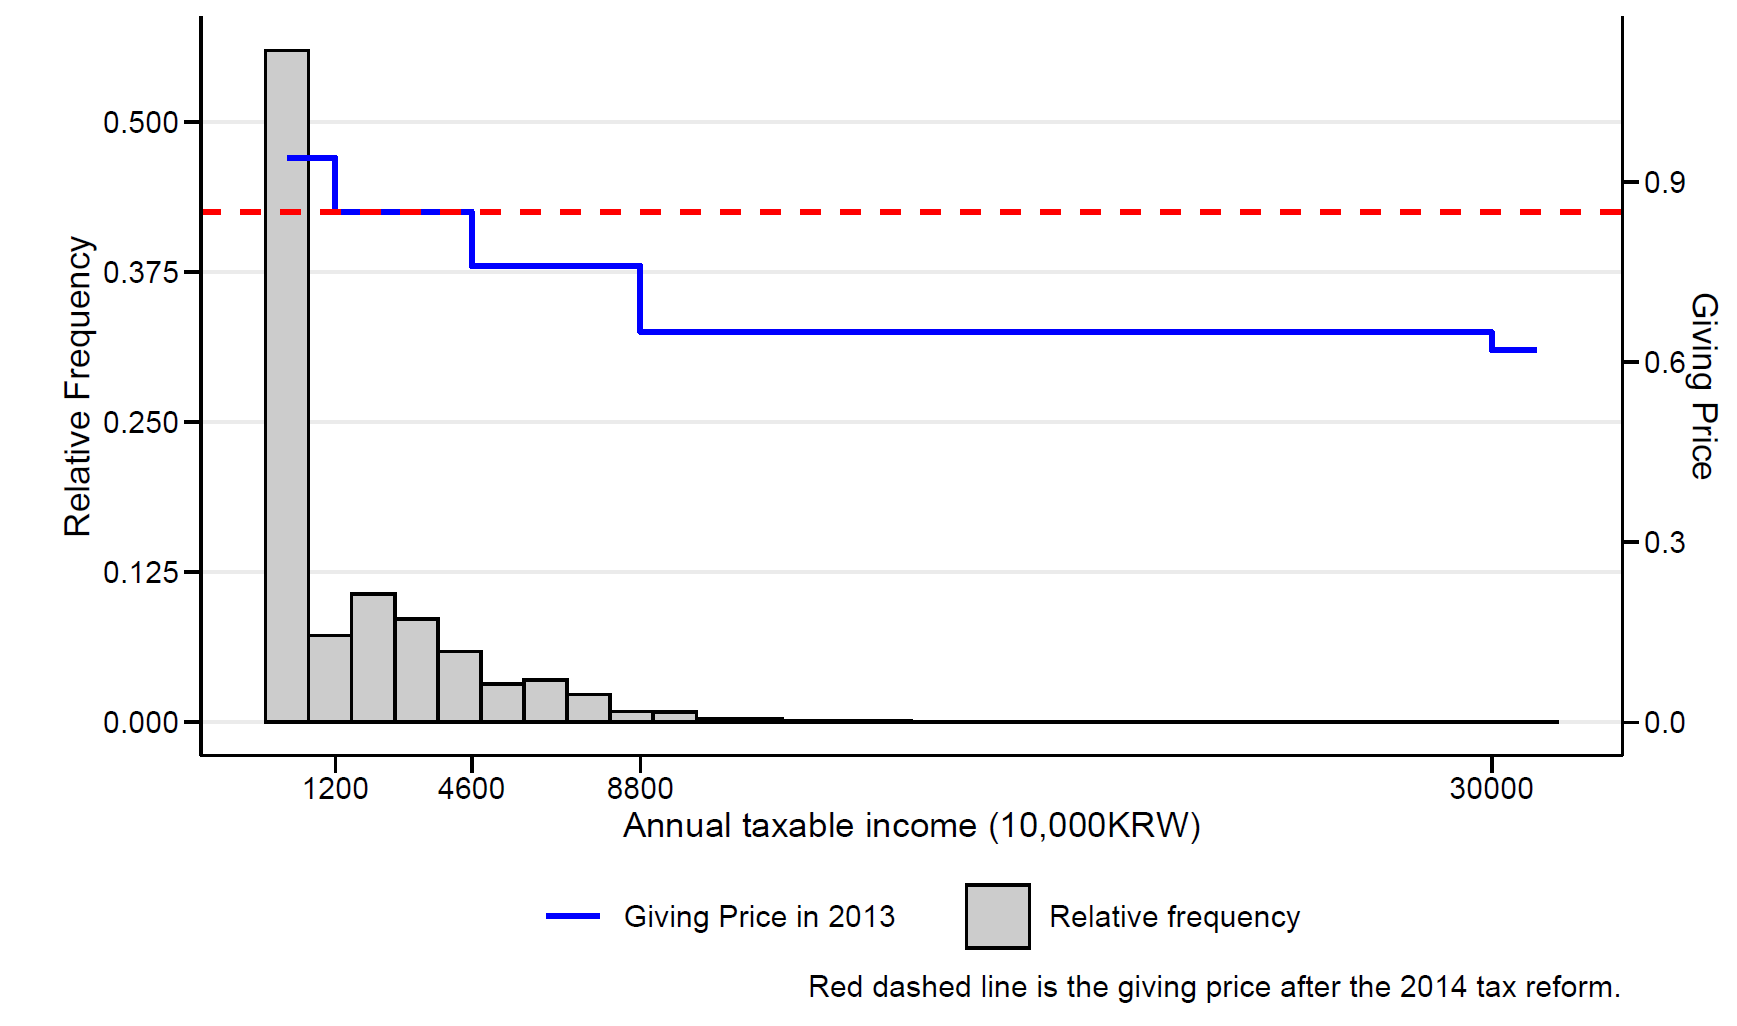
\includegraphics[width=0.7\linewidth]{Fig_Income_distribution}
		\caption{所得分布と税制改正前後での寄付価格の変化}
		\label{fig:2}
	\end{figure}
	\small
	2014年に寄付価格は概ね
	\begin{itemize}
		\item 所得1200万KRW未満の人については減少
		\item 所得1200万KRW$\sim$4600万KRWの人については同じ
		\item 所得4600万KRW以上の人については増加
	\end{itemize}
\end{frame}
	
	\begin{frame}{内生性の問題}
		\begin{enumerate}
			\item 課税申告データの使用は申告された寄付額のみを捉えることとなる。
			\begin{itemize}
				\item 未申告の寄付に寄付の税制優遇は無意味のはず(=推定バイアスに繋がる)
				\item 先行研究ではサーベイデータでこの問題に対処 (e.g.~Rehavi and Shack, 2013).
				\item \textbf{本稿でも韓国のサーベイデータでこの問題に対処。}
			\end{itemize}
			\item 申告コストが無視されると推定バイアスが発生する可能性。
			\begin{itemize}
				\item 申告コストが安くて寄付価格が安くなる人だけを捉えて推定する可能性(Self-selectionバイアス)
				\item 知る限りAlmunia et al.~(2020)のみが申告コストを考慮しているが、課税申告データを使用してしまっている。
				\item\textbf{本稿では給与所得者と非給与所得者の違いを操作変数(IV)として採用し、申告コストを考慮。}
			\end{itemize}
		\end{enumerate}
	\end{frame}
	
	\begin{frame}{Data}
		使用するデータは韓国のNational Survey of Tax and Benefit(NaSTab)のデータ
		\begin{itemize}
			\item このデータの対象は韓国全体の15の市と地域の一般世帯とその構成員。
			\item データは主に対面のインタビュー形式で回答されたもの。
			\item データサンプルは韓国の一般的な社会構成が代表されるように構成されている。
			\item 本稿では所得や資産がないと思われる23歳以下のサンプルは除いて分析している。
			\item データとして2012$\sim$2017年のデータを使用。(2014年の制度改正に着目)
		\end{itemize}
	\end{frame}

\begin{frame}{Data}
	\begin{figure}
		\centering
		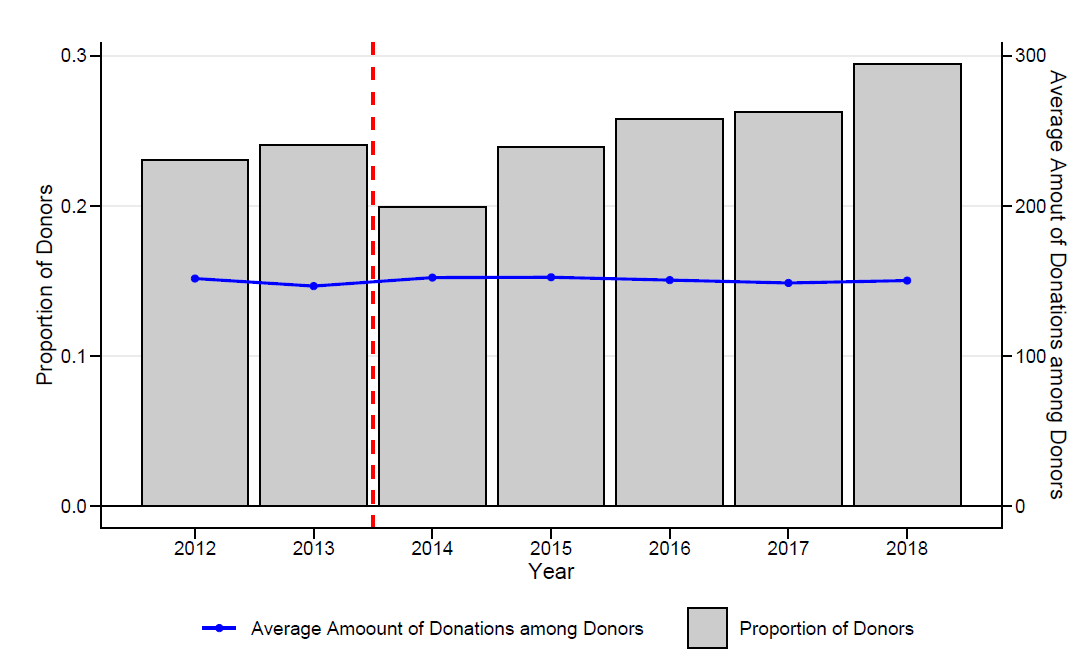
\includegraphics[width=0.8\linewidth]{Fig_Average_donation}
		\caption{寄付者の割合と寄付者の平均寄付額}
		\label{fig:1}
	\end{figure}
\small
	\begin{itemize}
		\item 20$\sim$30\%の人が寄付を実施
		\item 寄付者の平均寄付額は150万KRW($\simeq$15万円)程度
	\end{itemize}
\end{frame}



\begin{frame}{Data}
	\begin{figure}
		\centering
		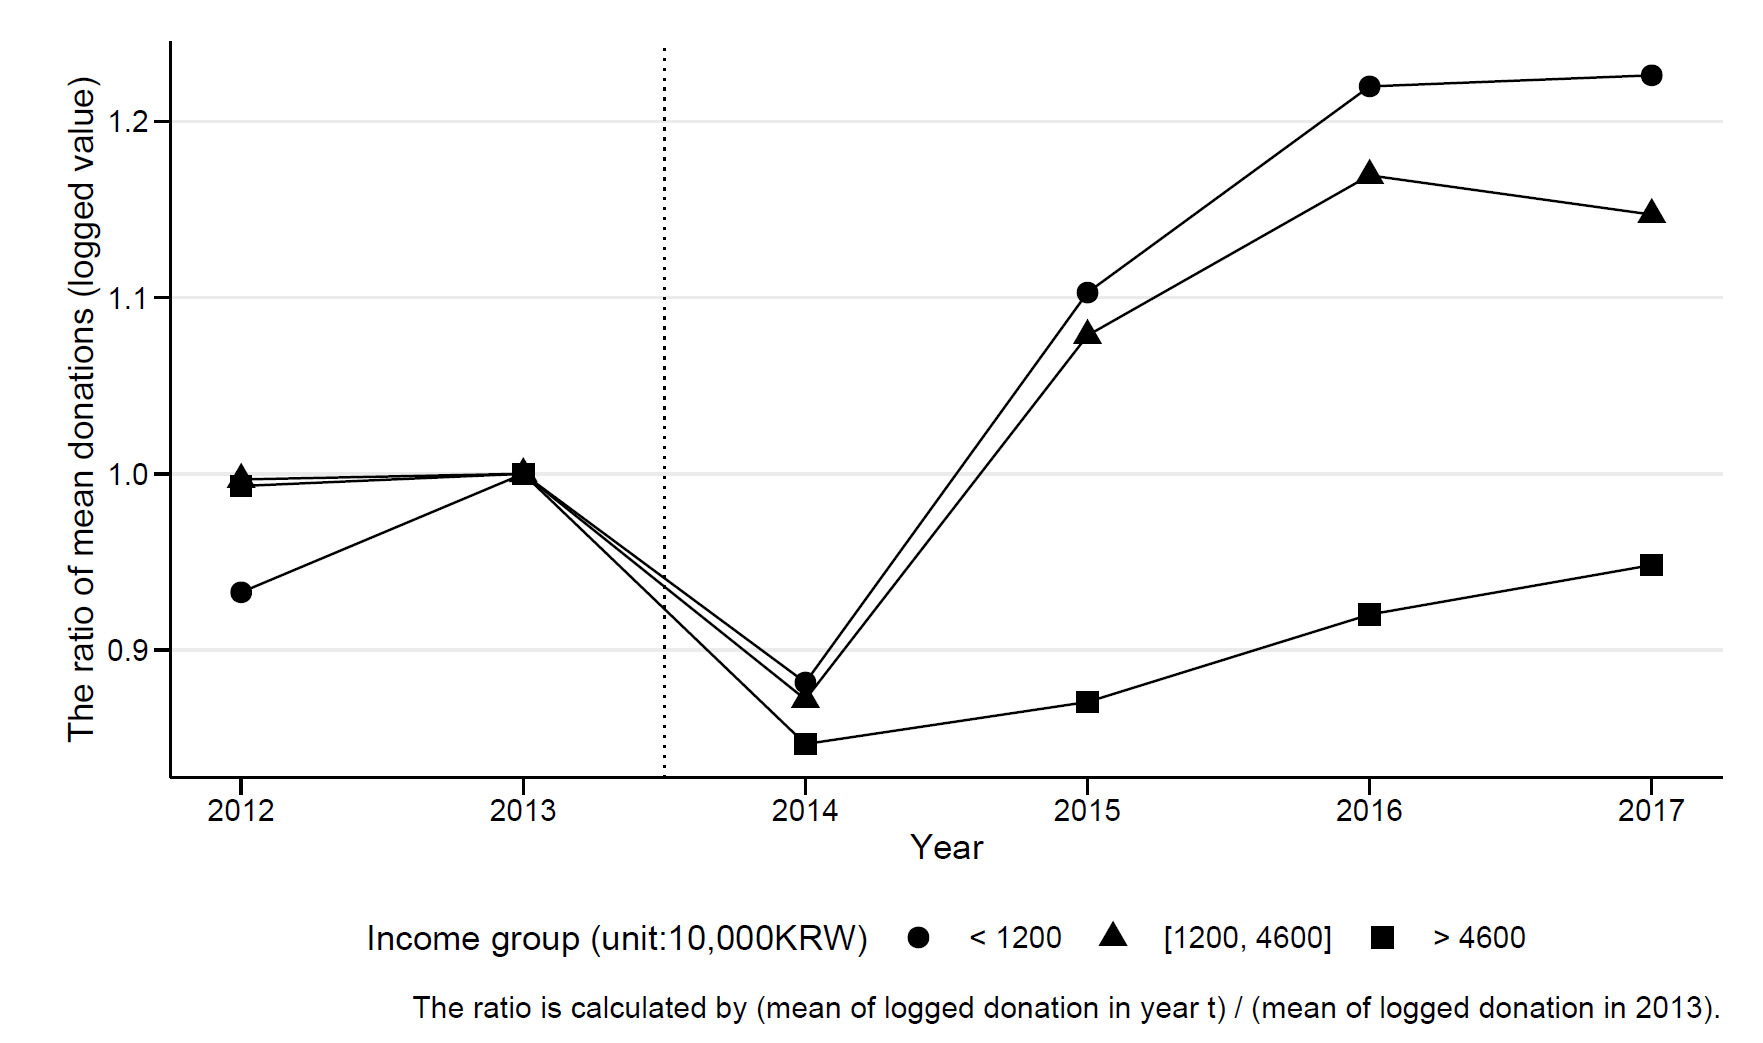
\includegraphics[width=0.7\linewidth]{Fig_Diff}
		\caption{各所得グループでの平均寄付額(対数)}
		\label{fig:3}
	\end{figure}
\small
	2012年と2013年に比べ、2014年以降の寄付額は
	\begin{itemize}
		\item 所得1200万KRW未満の人については増加
		\item 所得1200万KRW$\sim$4600万KRWの人についてはやや増加
		\item 所得4600万KRW以上の人については減少
	\end{itemize}
\end{frame}

\begin{frame}{Data}
	\begin{figure}
		\centering
		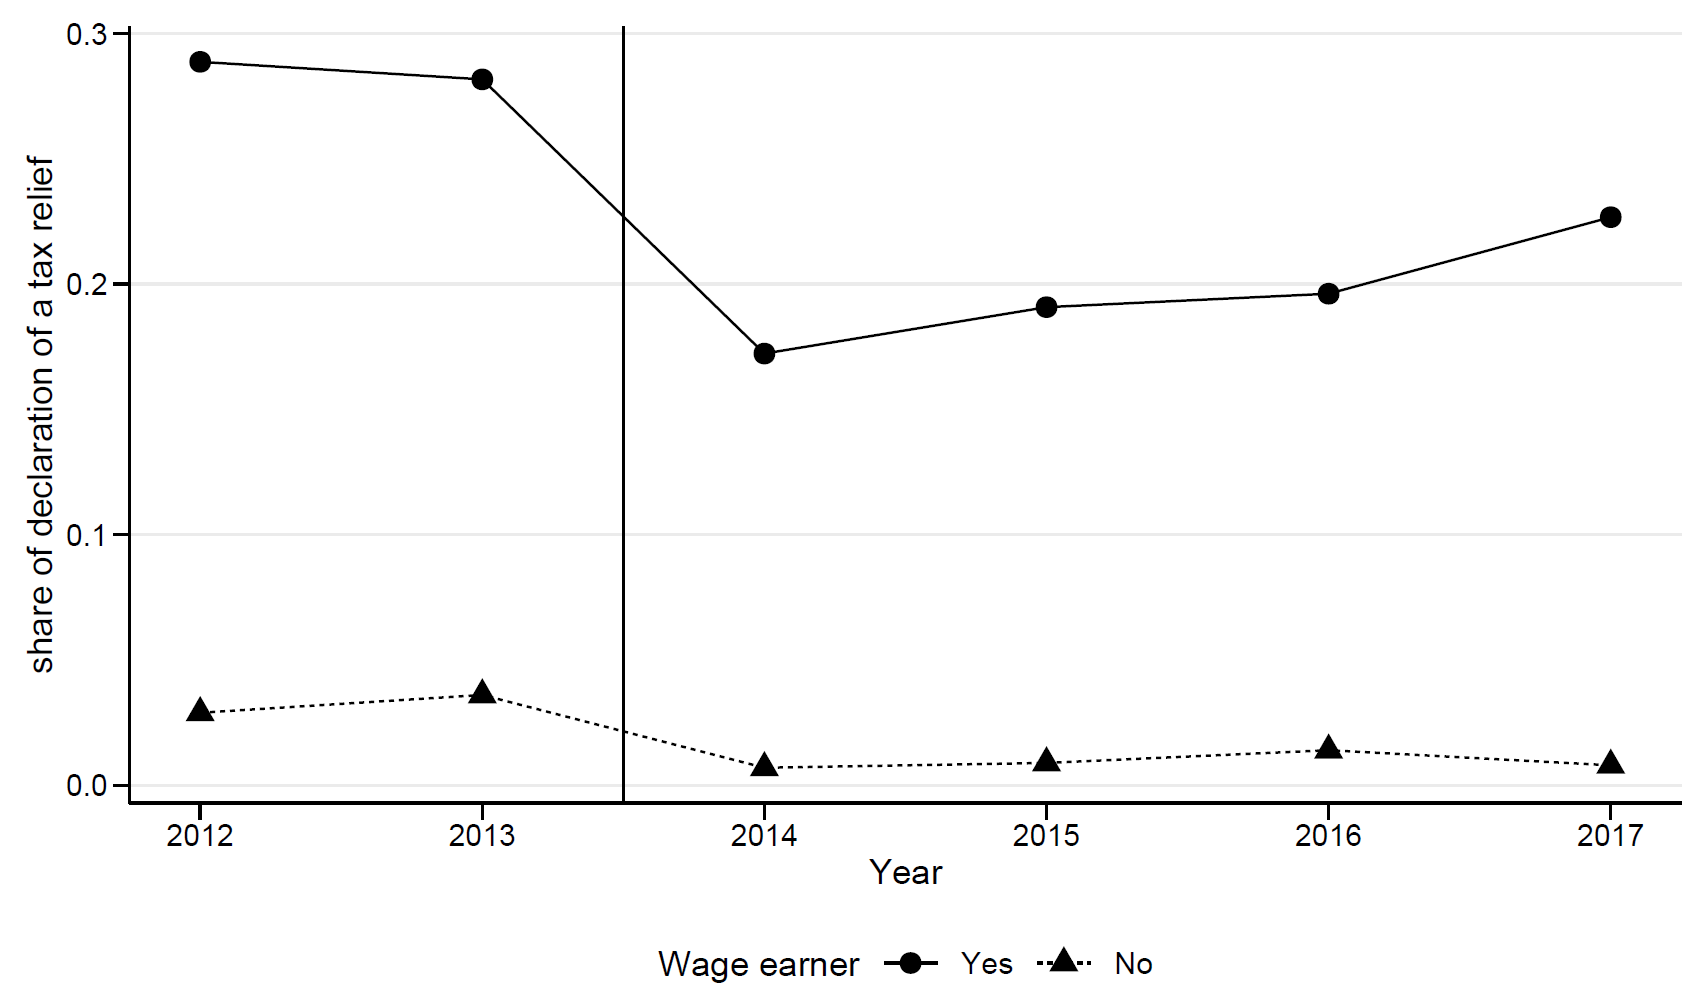
\includegraphics[width=0.7\linewidth]{Fig_Declaration}
		\caption{寄付申告者の割合}
		\label{fig:4}
	\end{figure}
\small
	\begin{itemize}
		\item 給与所得者は税制優遇を受けるため、より寄付の申告を行う傾向があるとわかる。\\
		$\to$ これは申告コストの違いを捉えたものだと考えられる。
	\end{itemize}
\end{frame}

\begin{frame}{Data}
	\begin{table}
		\centering
		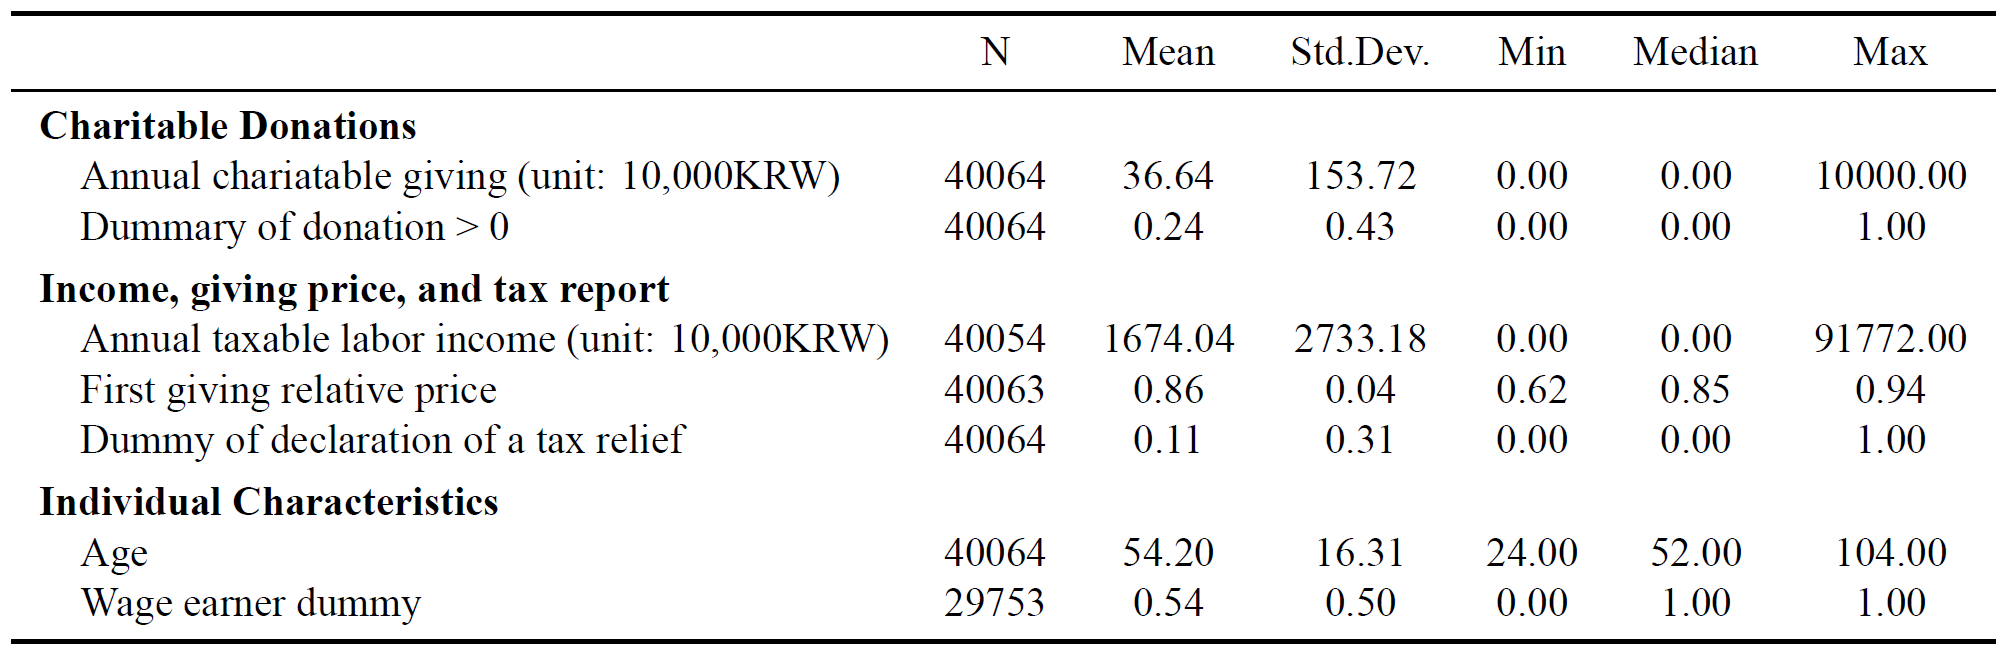
\includegraphics[width=0.9\linewidth]{Tab_Stat}
		\caption{基本統計量}
		\label{tab:1}
	\end{table}
\end{frame}

\begin{frame}{推定モデル}
\begin{itemize}
	\item 主な識別戦略として2014年の税制改正を使い、DIDに準じた推定を行う。
	\begin{itemize}
		\item 所得1200万KRW未満:寄付価格は減少
		\item 所得1200万KRW$\sim$4600万KRW:寄付価格は同じ
		\item 所得4600万KRW以上:寄付価格は増加
	\end{itemize}
	\item さらに申告コストの差の影響を捉えるために、サンプルが給与所得者かどうかをみるダミーをIVとして使用。
\end{itemize}
\end{frame}

\begin{frame}{推定モデル}
	\begin{itemize}
		\item 以下のような二元配置固定効果モデルを考える。
		\begin{align}
			\ln g_{it} = \varepsilon_pR_{it} \ln p_{it}(y_{it}, g_{it}) + \varepsilon_y \ln y_{it} + \bm{X}_{it}\bm{\beta} + \mu_i + \iota_t + u_{it}\tag{5}
		\end{align}
	$\mu_i, \iota_t$と$ u_{it}$はそれぞれ個人固定効果、年の固定効果、誤差項 
	\item $\bm{X}_{it}$は年齢の2乗、産業(職業)ダミー、地域ダミー
	\item 寄付の研究文脈では\textbf{intensive margins}と\textbf{extensive margins}を分けて弾力性を推定することが行われている。
	\begin{itemize}
		\item \textbf{Intensive margins}: (5)を寄付した個人($g_{it}>0$)に限定して分析\\
		$-$寄付価格の変化でどれくらいの量寄付が変化するかに関心
		\item \textbf{Extensive margins}: (5)の被説明変数を寄付するかどうか($1[g_{it}>0]$)にして分析\\
		$-$寄付価格の変化で寄付を行うようになるかどうかに関心
	\end{itemize}
	$\to$ 本稿ではこれらのどちらも分析
	\end{itemize}
\end{frame}

\begin{frame}{推定モデル: $p_{it}$の内生性}
	\begin{itemize}
		\item (私的財\$1と比較した)寄付の価格は
		\begin{align}
			p_{it}(y_{it}, g_{it})=\begin{cases}
			1-T'_t(y_{it}-g_{it})&\text{ if }t<2014\\
			0.85&\text{ if }t\ge2014
			\end{cases}
			\tag{6'}.
		\end{align}
		\item 2014年より前は寄付価格が寄付額に依存し、内生的となってしまうため、``\textbf{first-price of giving}"と呼ばれる寄付額が0の状態の寄付価格
		\begin{align}
			p_{it}^f(y_{it})=p_{it}(y_{it},0)\notag
		\end{align}
		を実際の寄付価格$p_{it}(y_{it},0)$の代わりに使用
		\item 実際の寄付価格$p_{it}(y_{it},0)$は``last-price of giving"と呼ばれ、これについても分析し頑健性を確認。
	\end{itemize}
\end{frame}

\begin{frame}{推定モデル: 寄付申告$R_{it}$の内生性}
	\begin{itemize}
		\item 寄付者は寄付を申告するかどうかを自ら選択できるため、寄付申告$R_{it}$は内生的となる。
		\item そのため、給与所得者ダミー$WageEarner_{it}$を寄付申告$R_{it}$の操作変数として用い、以下を分析。
		\begin{align}
			\ln g_{it} = \varepsilon_pR_{it} \ln p_{it}^f(y_{it}) + \varepsilon_y \ln y_{it} + \bm{X}_{it}\bm{\beta} + \mu_i + \iota_t + u_{it}\tag{7}
		\end{align} 
	 	\begin{itemize}
	 		\item 2段階最小二乗法(2SLS)に基づく推定
			\item 給与所得者ダミー$WageEarner_{it}$は所得や職業ダミーをコントロールした上では誤差項$u_{it}$とは相関しないと考えられる。
		\end{itemize}
	\end{itemize}
\end{frame}

\begin{frame}{推定モデル: 寄付申告$R_{it}$の内生性}
	\begin{itemize}
		\item 2SLSに加え、寄付申告の傾向スコア$P(Z_{it})$を操作変数として用いた推定も実施
		\begin{itemize}
			\item この方法は``control function (CF)"アプローチと呼ばれる。
			\item 傾向スコアは以下のプロビットモデルで推定
			\begin{align}
				R_{it}=1[\delta_0+Z_{it}\delta_1+u_{it1}>0]\tag{8},
			\end{align}
			ただし$Z_{it}\equiv \{WageEarner_{it}, \ln p_{it}^f(y_{it}), \ln y_{it}, \bm{X}_{it}\}$.
			\item 傾向スコアは$P(Z_{it})=\Phi(\hat{\delta}_0+Z_{it}\hat{\delta}_1)$となる。
			\item 2つの異なる仮定に基づいて別々の分析を実施\\
			 \ajMaru1 Pooledプロビット:係数$\delta\equiv (\delta_0, \delta_1)$が時間を通じて一定\\
			 \ajMaru2 Separatedプロビット:係数$\delta\equiv (\delta_0, \delta_1)$が時間で可変
		\end{itemize}
		\item さらに、寄付申告$R_{it}$の代わりに傾向スコアを直接使った分析も実施
		\begin{align}
			\ln g_{it} = \varepsilon_pP(Z_{it})\ln p_{it}^f(y_{it}) + \varepsilon_y \ln y_{it} + \bm{X}_{it}\bm{\beta} + \mu_i + \iota_t + u_{it}\tag{9}
		\end{align}
	\end{itemize}
\end{frame}

\begin{frame}{結果: Intensive Margins}
	\begin{table}
		\centering
		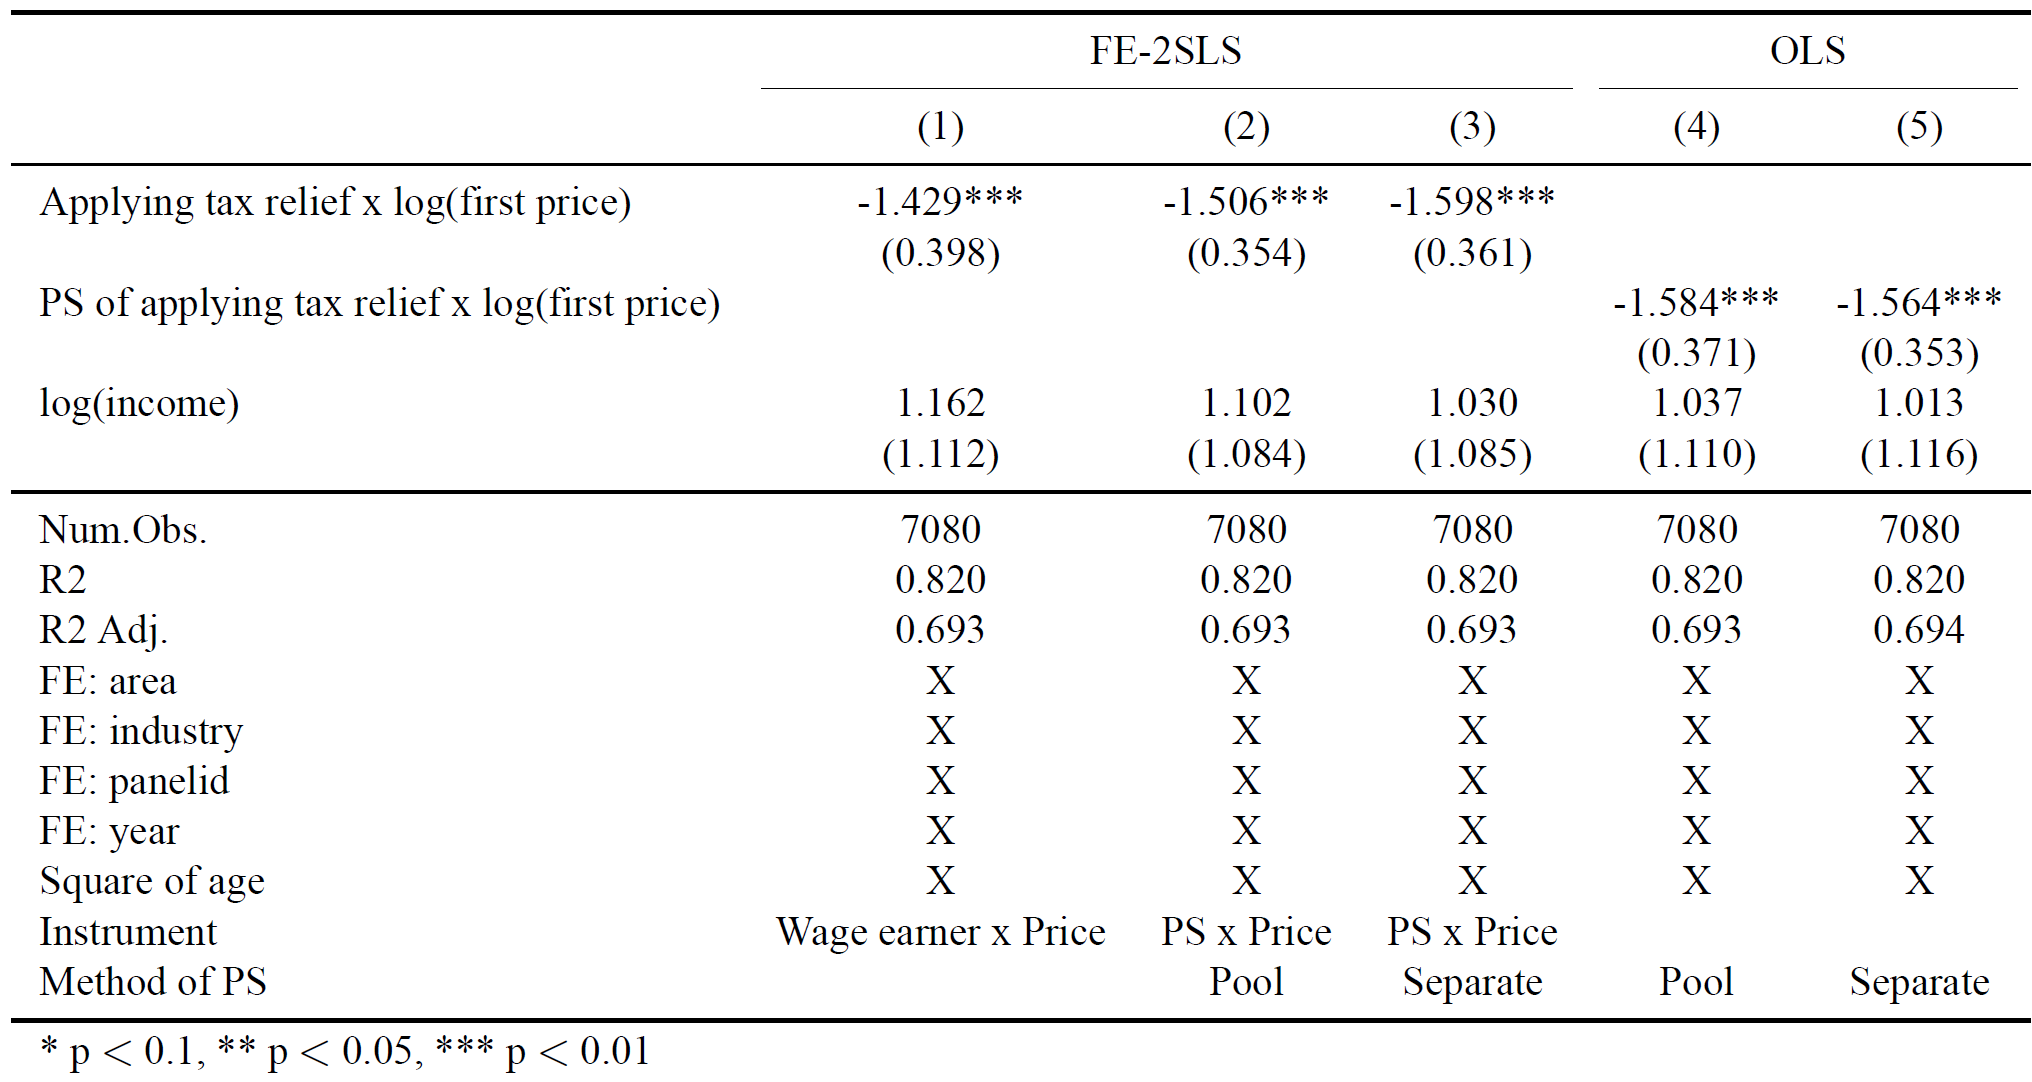
\includegraphics[width=0.9\linewidth]{Tab_res_1}
		\caption{First-Price Elasticities (Intensive Margins)}
		\label{tab:2}
	\end{table}
Intensive marginsでの寄付の価格弾力性の推定値は概ね-1.5程度となった。\\
(申告コストを考慮しない通常のモデルでの推定値は-0.91)
\end{frame}

\begin{frame}{結果: Extensive Margins}
	\begin{table}
		\centering
		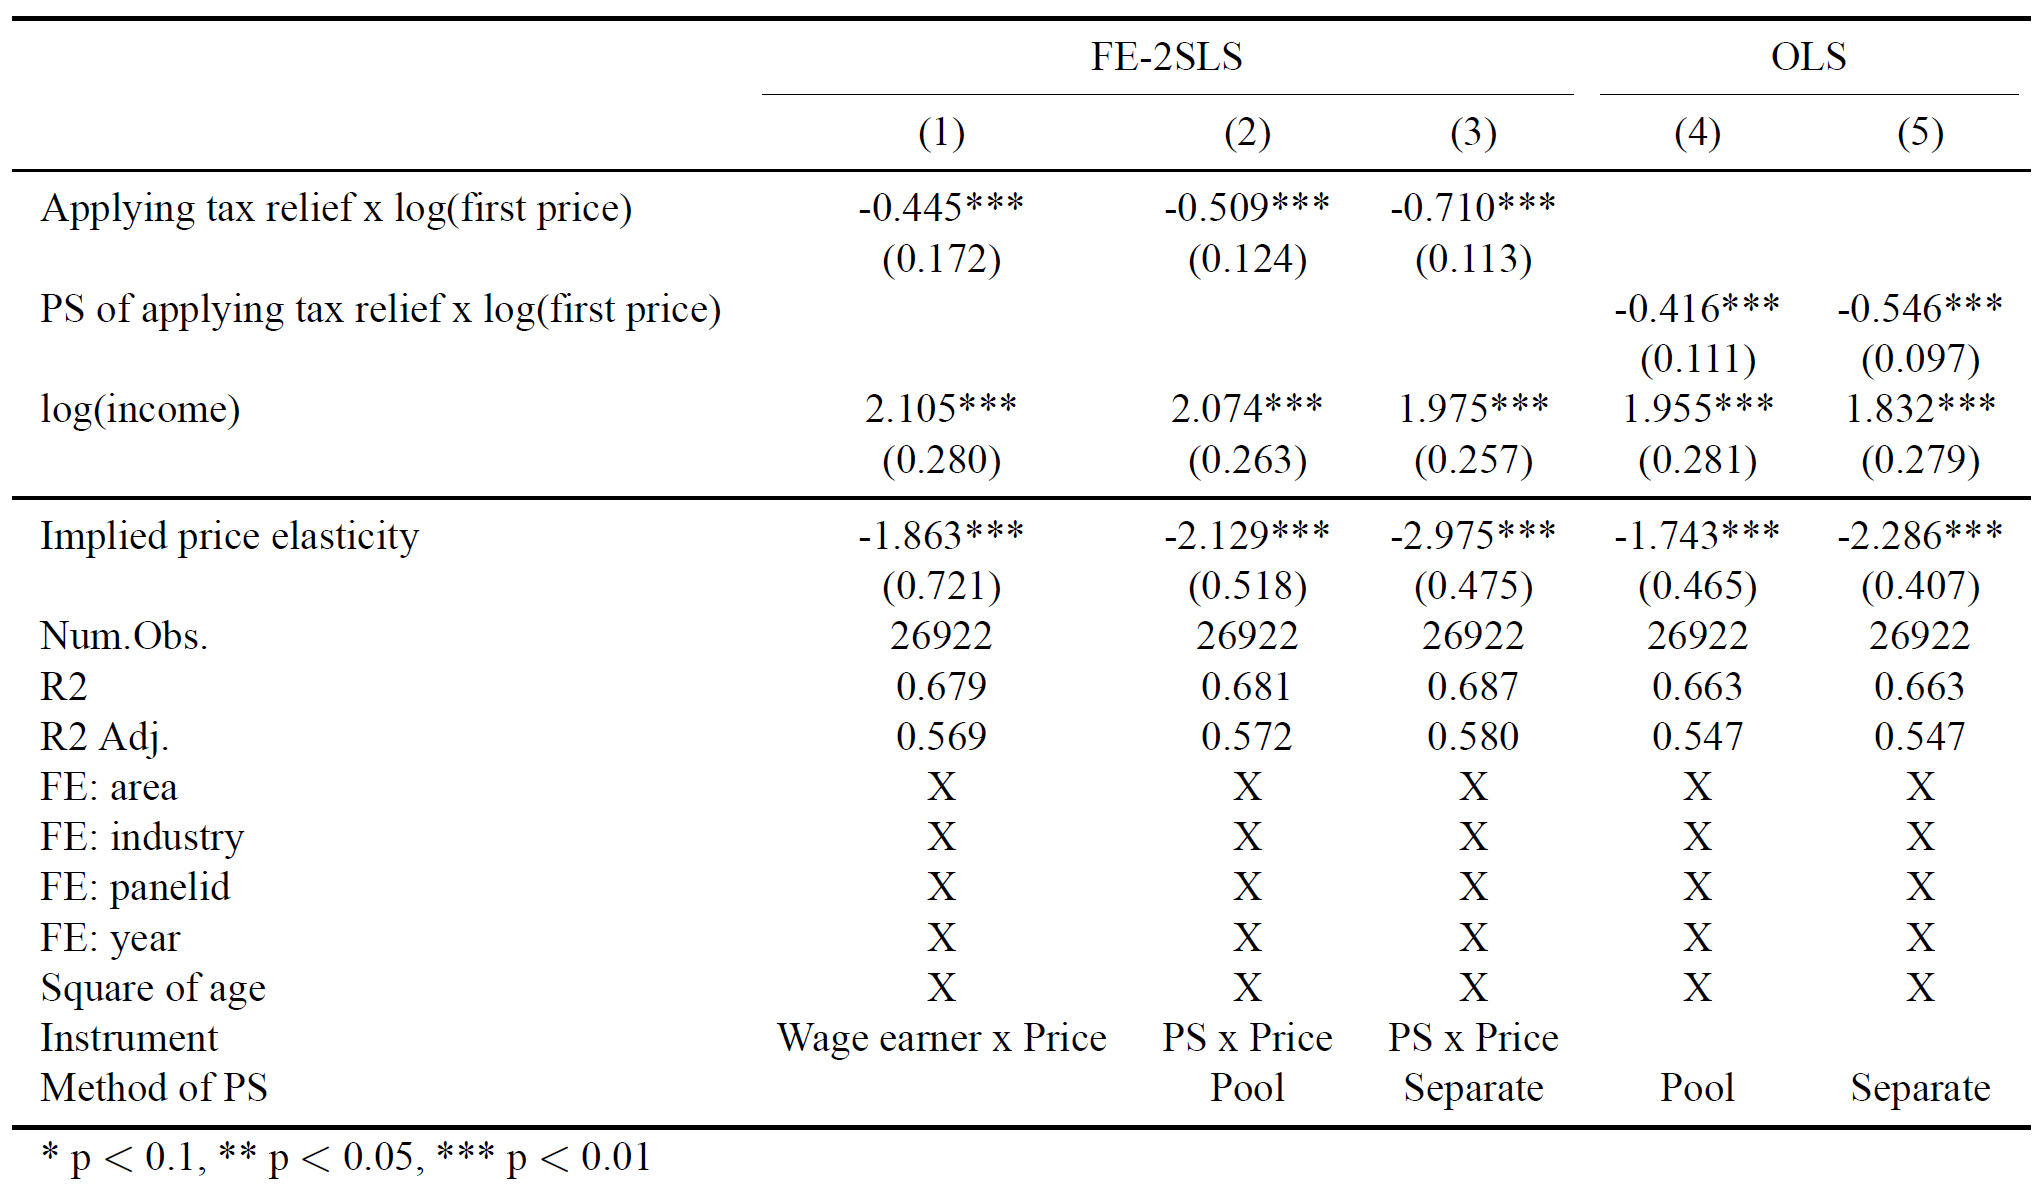
\includegraphics[width=0.9\linewidth]{Tab_res_2}
		\caption{First-Price Elasticities (Extensive Margins)}
		\label{tab:3}
	\end{table}
	Intensive marginsでの寄付の価格弾力性の推定値は概ね-1.7 $\sim$ -2.9となった。
\end{frame}

\begin{frame}{結果}
	\begin{itemize}
		\item 分析結果から韓国での寄付の価格弾力性は多くの先行研究で示された値より弾力的であることがわかった。
		\begin{itemize}
			\item 多くの先行研究ではIntensive Marginsの寄付の価格弾力性は-1程度
			\item 申告コストをIVに使用しない分析では-0.91となったため、申告コストの無視で過小推定になった可能性
		  	\item Extensive Marginsの寄付の価格弾力性についても先行研究と比べかなり弾力的な値\\
		  	e.g. Almunia et al.(2020)は最も弾力的な値で-0.73\\
		  	e.g. Backus and Grant (2019)では統計的に有意でなく、概ね0
		  \end{itemize}
	\end{itemize}
\end{frame}

\begin{frame}{結果:ロバストネスチェック}
 様々なロバストネスチェックを実施
		\begin{enumerate}
			\item 2013,2014年をOmit:税制改正のアナウンスメント効果を除去
			\item First priceでなく、Last priceで分析
			\item 寄付申告者に限定したサブサンプルによる分析
			\begin{itemize}
				\item Semykina and Wooldridge (2010)のsample selection bias除去の方法を利用
				\item Intensive marginsの寄付の価格弾力性は概ね-1.2\(\sim\)-1.6.
				\item 寄付申告者に限定することで所得控除制度による内生性を考えたロバストネスチェックを実施可能\\
				e.g. 所得の変動 (Randolph, 1995, and so on.)\\
				$\to$ k-thの階差モデル / リード・ラグの使用  
			\end{itemize}
		\end{enumerate}
		ほとんどの分析結果で寄付の価格弾力性が
		\begin{itemize}
			\item Intensive Marginsで-1.4以下 
			\item Extensive Marginsで-1.7以下
		\end{itemize}
		\flushright{となるとわかった。}
\end{frame}

\begin{frame}{社会厚生への含意}
	Almunia et al. (2020)にならい、個人の効用関数を特定化し、以下の最適化問題を考える。
	\begin{align}
		\max_{x_i,g_i,R_i}&U(x_i,g_i,G)= x_i - R_iK +\theta u(g_i) + V(G)\notag\\
		\text{s.t. }&x_i + g_i = R_i(y-T(y, g_i)) + (1-R_i)(y-T(y)),\notag\\
		&\text{ and }G=g_i+G_{-i}\notag,
	\end{align}
	ただし$\theta\in[\underline{\theta},\bar{\theta}$]は寄付選好で密度$f(\cdot)$に従う。 
	\begin{itemize}
		\item $G$は政府供給も含めた社会の寄付総量。
		\item $G_{-i}$は社会の寄付総量から$i$の寄付を除いたもの。
		\item 簡単化のため、所得税は線形で税率$\tau$とする。
	\end{itemize}
\end{frame}

\begin{frame}{社会厚生への含}
	\begin{itemize}
	\item 最適化問題の結果、寄付者のうち寄付申告をする人としない人の(寄付に関する)間接効用関数はそれぞれ以下のようになる。
	\begin{align}
		\nu(p;\theta)&=\theta_i u(g(p;\theta))-pg(p;\theta)\notag\\
		\nu(1;\theta)&=\theta_i u(g(1;\theta))-g(1;\theta)\notag.
	\end{align}
\end{itemize}
\end{frame}

\begin{frame}{社会厚生への含意}
	\begin{itemize}
		\item 寄付選好$\theta$と寄付価格$p$の大きさによって社会には以下の3種類の人が存在。
		\begin{enumerate}
			\item 非寄付者: $\theta\le \theta_0$
			\item 寄付者かつ非寄付申告者: $\theta\in(\theta_0,\theta(p)]$\\
			$\to$ 彼らの寄付総額を$g^0(p)\equiv\int_{\theta_0}^{\theta(p)}g(1;\theta)f(\theta)d\theta$とする。
			\item 寄付者かつ寄付申告者: $\theta>\theta(p)$\\
			$\to$ 彼らの寄付総額を$g^1(p)\equiv\int_{\theta(q)}^{\bar{\theta}}g(p;\theta)f(\theta)d\theta$とする。
		\end{enumerate}
	\item 社会厚生は以下のようになる。
	\begin{align}
		W=V(G)&+\int_{\theta(p)}^{\bar{\theta}}(\nu(p;\theta)-K)f(\theta)d\theta\notag\\
		&+\int_{\theta_0}^{\theta(p)}\nu(1;\theta)f(\theta)d\theta+\lambda[ty-(1-p)g^1(p)-G_g]\notag
	\end{align}
	ただし$\lambda$は公的資金の限界費用(MCPF)を表す。
	\item 政府はMCPFと公共財の限界効用が等しくなるように公共財を供給し$\lambda=V'$となる(Saez, 2004)。
	\end{itemize}
\end{frame}

\begin{frame}{社会厚生への含意}
	\begin{itemize}
		\item 寄付価格$p$を変化させたときの社会厚生$W$の変化を考えると
		\begin{align}
			\frac{dW}{dp} =\lambda (g_p^0+g_p^1)+(\lambda-1)g^1-\lambda(1-p)g_p^1\notag
		\end{align}
		\item 寄付価格を下げたときに社会厚生が上がる$\frac{dW}{dp}<0$の条件は以下と同値
		\begin{align}
			\epsilon\equiv -\frac{pg_p^1}{g^1}>\frac{\lambda-1}{\lambda}+\frac{g_p^0}{g^1}\notag.
		\end{align}
		\begin{itemize}
		\item サブサンプル分析より$\epsilon$は1.304 $\sim$ 1.603
		\item MCPFは$\lambda\in[1,2]$だと仮定し、$\frac{\lambda-1}{\lambda}\in[0,\frac12]$となる。
		\item データから$\frac{g_p^0}{g^1}$は0.22 $\sim$ 0.34
		\end{itemize}
		\item これらより、$\frac{dW}{dp}<0$がいえ、寄付価格を下げたときに社会厚生が上がると示唆される。
	\end{itemize}
\end{frame}



\begin{frame}{寄付申告の差による寄付額の差}
	\begin{itemize}
		\item Wooldridge(2015)よりCFアプローチをもとに、寄付申告の傾向スコア算出時のプロビット推定を使い、寄付申告を行うことによる寄付の増大がどれくらいになるかを算出
		\item プロビット推定で得られた$\hat{\delta}$と逆ミルズ比$\Lambda(\cdot)$を使い、以下を算出
		\begin{align}
			\hat{r}_{it}\equiv R_{it}\Lambda(Z_{it}\hat{\delta})-(1-R_{it})\Lambda(Z_{it}\hat{\delta})\notag
		\end{align}
		\item $\hat{r}_{it}$は一般化残差といい、申告コストの差によるSelf-selectionを考慮
		\item 発想:内生変数$R_{it}$は誤差項と相関を持つのが問題\\
		\qquad$\to$$R_{it}$と残差との相関を捉えた項を説明変数とすれば問題ない
		\item ここでの主な識別源は$Z_{it}$に含まれる給与所得者ダミー
	\end{itemize}
\end{frame}


\begin{frame}{寄付申告の差による寄付額の差}
一般化残差を説明変数に加えた次の推定式を寄付者を対象に以下のように実行
		\begin{align}
			\ln g_{it} = \varepsilon_p\ln p_{it}+\varepsilon_y \ln y_{it} + \bm{X}_{it}\bm{\beta} + \mu_i + \iota_t + \hat{r}_{it}+u_{it}\notag
		\end{align}
		\begin{enumerate}
			\item 寄付申告者$R_{it}=1$の個体について上記の回帰を実施。
			\item 非寄付申告者$R_{it}=0$の個体について上記の回帰を実施。
			\item 分析1と2で得た係数から、すべての個体を使って$R_{it}=0$だった場合の予測値$\ln g_{it}^{(0)}$と$R_{it}=1$だった場合の予測値$\ln g_{it}^{(1)}$を得る。
			\item 以下の値を算出
			\begin{itemize}
				\item $\hat{ATE}\equiv N^{-1}\sum_{i=1}^N[\ln g_{it}^{(1)}-\ln g_{it}^{(0)}]$
				\item $\hat{ATT}\equiv N_1^{-1}\sum_{i=1}^NR_{i1}[\ln g_{it}^{(1)}-\ln g_{it}^{(0)}]$
				\item $\hat{ATU}\equiv N_0^{-1}\sum_{i=1}^N(1-R_{i1})[\ln g_{it}^{(1)}-\ln g_{it}^{(0)}]$
			\end{itemize}
			ただし$N$は全サンプル数、$N_1(N_0)$は(非)寄付申告者のサンプル数
		\end{enumerate}
	\end{frame}

\begin{frame}{寄付申告の差による寄付額の差}
	\begin{itemize}
		\item 寄付者が非寄付申告者から寄付申告者となったときの寄付の増加$d \ln g$は以下のように推定された。
		\begin{itemize}
			\item 寄付者全体での平均効果(ATE): 0.201\\
			$\to$ 今よりも20.1ppt寄付額が増加
			\item 寄付者のうち申告者での平均効果(ATT): 0.295\\
			$\to$ 今よりも29.5ppt寄付額が増加
			\item 寄付者のうち非申告者での平均効果(ATU): 0.138\\
			$\to$ 今よりも13.8ppt寄付額が増加
		\end{itemize}
		(※Pooled Probitの仮定を行った場合での推定結果)
		\item 寄付申告で税制優遇が受けられるようになったことで概ね20pptほど寄付額が増加することがわかる。
	\end{itemize}
\end{frame}

	\begin{frame}{Conclusion}
	分析の結果
	\begin{enumerate}
		\item ベースラインの結果では、寄付の価格弾力性がIntensive Marginsで-1.4以下、Extensive Marginsで-1.7以下となった。
		\begin{itemize}
			\item 寄付の申告コストを考慮しない結果ではIntensive Marginsで-0.9となった。
		\end{itemize}
		\item 寄付の申告者に絞った分析結果では寄付の価格弾力性はIntensive Marginsで-1.2\(\sim\)-1.6となった。
	\end{enumerate}
	既存研究の多くではIntensive Marginsの寄付の価格弾力性が約-1であり、これよりも概ね弾力的な推定結果が得られた。
	\begin{enumerate}
		\setcounter{enumi}{2}
		\item 推定値をもとに社会厚生を分析すると韓国では寄付の税制優遇を拡充することで厚生が増大する可能性が高いことがわかった。
		\item 寄付の申告が行われることによる寄付の増加は概ね20\%程度だとCFアプローチからわかった。
	\end{enumerate}
\end{frame}
\end{document}